%Adjust the path to the posters/ directory here
\documentclass[final,a0paper]{poster/ivtposter}
%\documentclass[final,trb]{ivtposter}
%\documentclass[a4shrink,portrait,final]{ivtposter}
% Use a4shrink for an a4 sized paper.

% All files are supposed to be in UTF-8 now:
% (ENCODING CHECK: äöüÄÖÜßéàè)

% You probably need to change this
\usepackage[latin]{babel}%

\usepackage{booktabs}
\usepackage{graphicx}
\usepackage{amsmath}
\usepackage{cleveref}
\usepackage{sansmath}
\usepackage{amsfonts}
\usepackage[backend=bibtex,style=authoryear,natbib=true]{biblatex}

\addbibresource{bib.bib}

%% To use the FF DIN Pro font:
\iffalse
\usepackage{fontspec}
\setmainfont[BoldFont=*-Bold, ItalicFont=*-Italic, BoldItalicFont=*-BoldItalic, Ligatures=TeX, Numbers=OldStyle]{DINPro}
\usepackage{unicode-math}
\setmathfont{Asana Math} % for math symbols, can be any other OpenType math font
\setmathfont[Ligatures=TeX, Numbers={Lining,Proportional}, range=\mathup]  {DINPro}
\setmathfont[Ligatures=TeX, Numbers={Lining,Proportional}, range=\mathbfup]  {DINPro}
\setmathfont[Ligatures=TeX, Numbers={Lining,Proportional}, range=\mathbfit]  {DINPro-BoldItalic}
\setmathfont[Ligatures=TeX, Numbers={Lining,Proportional}, range=\mathit]{DINPro-Italic}
\fi

\tracingstats=2

\graphicspath{{poster/},{data/cond_gen}}
\DeclareGraphicsExtensions{.pdf,.eps,.png,.jpg}

\newcommand{\xset}{\mathbb{X}}
\newcommand{\xseti}{\mathbb{X}^{(i)}}
\newcommand{\approxdistri}{q_{\phi}(\textbf{z}|\xseti)}
\newcommand{\approxdistr}{q_{\phi}(\textbf{z}|\xset)}
\newcommand{\truedistr}{p_{\theta}(\textbf{z}|\xseti)}
\newcommand{\elbo}{\mathcal{L}(\theta, \phi; \xseti)}
\newcommand{\xsubset}{\mathbb{X}_k}
\newcommand{\lmopoe}{\mathcal{L}_{MoPoE}(\theta, \phi; \xset)}
\newcommand{\powerset}{\mathcal{P}(\xset)}

%%%%%%%%%%%%%%%%%%%%%%%%%%%%%%%%%%%%%%%%%%%%%%%%%%%%%%%%%%%%%%%%%%%%%%%%%%%%%%
%%% Begin of Document
%%%%%%%%%%%%%%%%%%%%%%%%%%%%%%%%%%%%%%%%%%%%%%%%%%%%%%%%%%%%%%%%%%%%%%%%%%%%%%

\begin{document}
%%%%%%%%%%%%%%%%%%%%%%%%%%%%%%%%%%%%%%%%%%%%%%%%%%%%%%%%%%%%%%%%%%%%%%%%%%%%%%
%%% Here starts the poster
%%%---------------------------------------------------------------------------
%%% Format it to your taste with the options
%%%%%%%%%%%%%%%%%%%%%%%%%%%%%%%%%%%%%%%%%%%%%%%%%%%%%%%%%%%%%%%%%%%%%%%%%%%%%%

    \typeout{Poster Starts}
    \begin{poster}%
    % Poster Options
    {
        columns=2, %1-6
    % Show grid to help with alignment
        grid=no
    }
    % Eye Catcher
    {} % No eye catcher for this poster. (eyecatcher=no above). If an eye catcher is present, the title is centered between eye-catcher and logo.
    % Title
    {~}
    % Authors
    {}
    % University logo
    {}

%%%%%%%%%%%%%%%%%%%%%%%%%%%%%%%%%%%%%%%%%%%%%%%%%%%%%%%%%%%%%%%%%%%%%%%%%%%%%%
%%% Now define the boxes that make up the poster
%%%---------------------------------------------------------------------------
%%% Each box has a name and can be placed absolutely or relatively.
%%% The only inconvenience is that you can only specify a relative position 
%%% towards an already declared box. So if you have a box attached to the 
%%% bottom, one to the top and a third one which should be in between, you 
%%% have to specify the top and bottom boxes before you specify the middle 
%%% box.
%%%%%%%%%%%%%%%%%%%%%%%%%%%%%%%%%%%%%%%%%%%%%%%%%%%%%%%%%%%%%%%%%%%%%%%%%%%%%%
        %
        % A coloured circle useful as a bullet with an adjustably strong filling
        \newcommand{\colouredcircle}[1]{%
            \tikz{\useasboundingbox (-0.2em,-0.32em) rectangle(0.2em,0.32em); \draw[draw=black,fill=baposterBGone!80!black!#1!white,line width=0.03em] (0,0) circle(0.18em);}}

        \headerbox{}{name=title,column=0,row=0,span=2,noheader=yes}{%
            \begin{flushleft}
                \setlength{\parskip}{1ex}
                {\fontsize{34.3}{41.2}\bfseries\selectfont
                Multimodal Generative Learning on the MIMIC-CXR Database
                \par
                }
                \vspace{1ex}
                {\Large
%                Subtitle that also should not be longer than 2 lines -- subtitle subtitle subtitle subtitle subtitle
%                subtitle subtitle subtitle subtitle subtitle subtitle subtitle subtitle
                \par
                }
                \vspace{2ex}
                {
                    \Large\bfseries
                    Hendrik Klug\textsuperscript{1+}\hspace{-.25em},
                    Thomas M. Sutter\textsuperscript{2}\hspace{-.25em},
                    Julia E. Vogt\textsuperscript{2}
                    \par
                }
                \textsuperscript{1}Department of Electrical Engineering, ETH Zürich;
                \textsuperscript{2}Department of Computer Science, ETH Zürich:
                \\
                \textsuperscript{+}Hendrik Klug; klugh@ethz.ch
            \end{flushleft}
        }

%%%%%%%%%%%%%%%%%%%%%%%%%%%%%%%%%%%%%%%%%%%%%%%%%%%%%%%%%%%%%%%%%%%%%%%%%%%%%%
        \headerbox{1 Introduction}{name=introduction,column=0,below=title}{
%%%%%%%%%%%%%%%%%%%%%%%%%%%%%%%%%%%%%%%%%%%%%%%%%%%%%%%%%%%%%%%%%%%%%%%%%%%%%%
            Machine Learning has become more and more popular in the medical domain over the past years.
            While supervised machine learning has already been applied successfully, the vast amount of unlabelled data
            offers new opportunities for un- and self-supervised learning methods.
            Especially with regard to the multimodal nature of most clinical data, the labelling of multiple data types
            becomes quickly infeasible in the medical domain.
            However, to the best of our knowledge, multimodal, unsupervised and generative methods have been tested
            extensively on toy-datasets only but have never been applied to real-world medical data, for direct
            applications such as disease classification and image generation.
            In this article, we demonstrate that this class of methods provides promising results on medical data while
            highlighting that the task is extremely challenging and
%            leaving space
            that there is space
            for substantial improvements.
        }

%%%%%%%%%%%%%%%%%%%%%%%%%%%%%%%%%%%%%%%%%%%%%%%%%%%%%%%%%%%%%%%%%%%%%%%%%%%%%%
        \headerbox{3 Results}{name=methods,column=0,below=introduction,above=bottom}{
%%%%%%%%%%%%%%%%%%%%%%%%%%%%%%%%%%%%%%%%%%%%%%%%%%%%%%%%%%%%%%%%%%%%%%%%%%%%%%
            \textbf{Evaluation of the latent representation.} We evaluate the ability of a linear classifier to classify subsets of different modalities according to the label "Finding". The evaluation with respect to every subset of modalities demonstrates the model's ability to infer meaningful representations in case of missing data types.
            \Cref{tab:lr_table} shows the performance for all subsets of the powerset $\powerset$.
%% For every subset, the classifier is trained and evaluated on the respective subset.
%the evaluation of linear classifiers that were trained on each of the inferred subsets of the powerset $\powerset$ from the training set and evaluated on the subsets that were inferred from the test set.
            The highest score is achieved if all three modalities are present.
            This demonstrates that the information of all modalities is successfully merged in the joint posterior distribution.
%\vspace{-0.15in}
%            \begin{table}[htbp]
%                \floatconts
%                {tab:lr_table}%
%                {\caption{\textbf{Classification results of the linear classifiers.}
%                We evaluate the ability of the classifiers to classify the learned representations of all subsets of modalities correctly.
%                The mean average precision over the test set is reported (F: frontal image, L: lateral image, T: text report).
%                %The random performance lies at 0.235.
%                }}%
%                {\begin{tabular}{lcccccccc}
%                     MODEL & F     & L     & T     & L,F   & F,T   & L,T   & L,F,T          \\
%                     \hline
%                     MoPoE & 0.467 & 0.460 & 0.473 & 0.476 & 0.493 & 0.475 & \textbf{0.494} \\
%                     Random & \multicolumn{6}{c}{0.235}
%                \end{tabular}}
%            \end{table}

            \textbf{Generation Quality.} \Cref{fig:fig_cond_lattext,fig:fig_cond_latPAtext} compare the generation quality of the model, with and without the F modality as input.
            Adding the F modality as input brings a significant improvement to the quality of the generated images.
            The generated samples from \Cref{fig:fig_cond_latPAtext} are less blurry and smaller details are recognisable.

            \createfigure{}{\textbf{Generated samples.} On the left, the L and T modality are given to the model as input. On the right, all modalities (F, L and T) are given as input.
            The samples above the red line are the input samples and those below are generated by the model.}{1}{%

                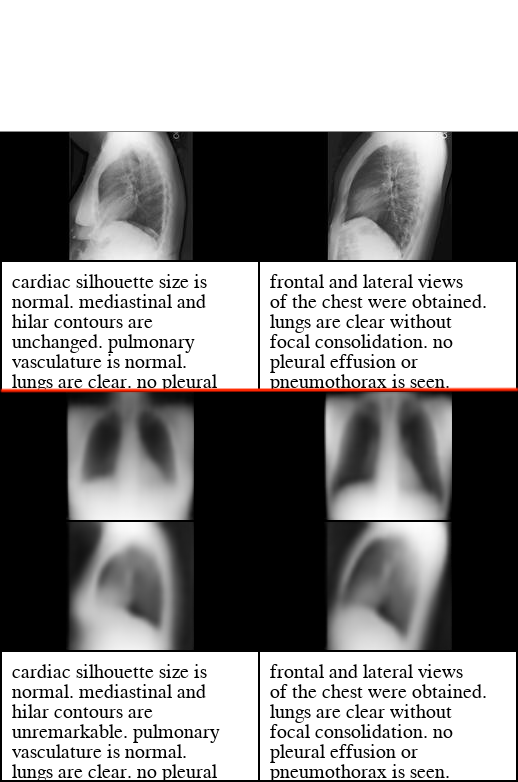
\includegraphics[width=0.49\linewidth]{data/cond_gen/Lateral_text_small_edited}
                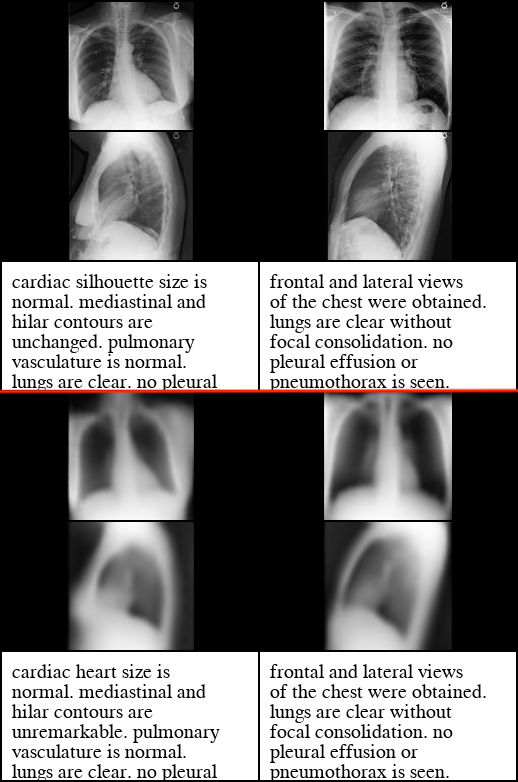
\includegraphics[width=0.49\linewidth]{data/cond_gen/Lateral_PA_text_small_edited}

            }{}
%
%            \begin{figure}[htbp]
%
%                \label{fig:cond_gen}% label for whole figure
%                \caption{\small{\textbf{Generated samples.} On the left, the L and T modality are given to the model as input. On the right, all modalities (F, L and T) are given as input.
%                The samples above the red line are the input samples and those below are generated by the model.}}% caption for whole figure
%                \begin{subfigure}
%                    \label{fig:fig_cond_lattext}
%                    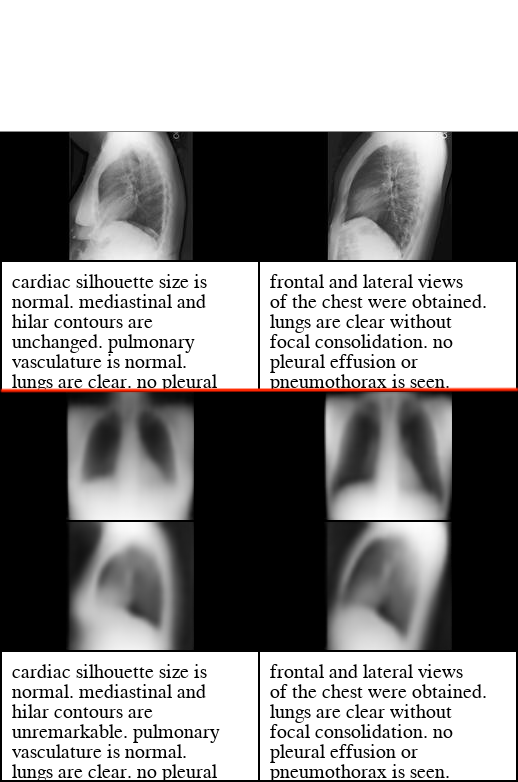
\includegraphics[width=0.3\linewidth]{data/cond_gen/Lateral_text_small_edited}
%                \end{subfigure}
%                \qquad % space out the images a bit
%                \begin{subfigure}
%                    \label{fig:fig_cond_latPAtext}
%                    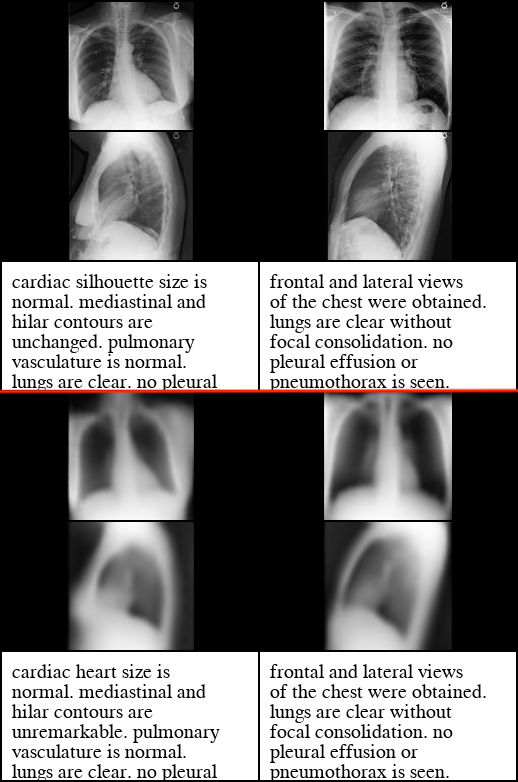
\includegraphics[width=0.3\linewidth]{data/cond_gen/Lateral_PA_text_small_edited}
%                \end{subfigure}
%            \end{figure}
        }

%%%%%%%%%%%%%%%%%%%%%%%%%%%%%%%%%%%%%%%%%%%%%%%%%%%%%%%%%%%%%%%%%%%%%%%%%%%%%%
        \headerbox{5 References}{name=references,column=1,above=bottom}{
%%%%%%%%%%%%%%%%%%%%%%%%%%%%%%%%%%%%%%%%%%%%%%%%%%%%%%%%%%%%%%%%%%%%%%%%%%%%%%
        \printbibliography
        }

%%%%%%%%%%%%%%%%%%%%%%%%%%%%%%%%%%%%%%%%%%%%%%%%%%%%%%%%%%%%%%%%%%%%%%%%%%%%%%
        \headerbox{4 Conclusion}{name=conclusion,column=1,above=references}{
%%%%%%%%%%%%%%%%%%%%%%%%%%%%%%%%%%%%%%%%%%%%%%%%%%%%%%%%%%%%%%%%%%%%%%%%%%%%%%
            Loruptiorem volorum volecte minis re, volecer epeditam faccaec ullabore deni-
            mus aut essimin velibus.

            Iliquiatus entemod quas modi ommoloris rae. Ut illutem similibus siti unt.

            Tem qui niende volorem voluptam quate nusape landiam endello remquid mi,
            quaspis re, si bea corro ipsanistisit la sit harci dolupta errores as magniendi odit
            et que pra sus aut aut illigen itatiis estionsedit ommodi atibus sam consedisqui
            rem hit perchil et officip iendae solorpo reratias mos modia doloreptaque inctur,
            aut volut rerchil inis acia volest rehent ad quibus expliti quam, quianto et parunt
            qui dolupti apernate abo. Bea nos iurem est, officitio dicia con enimiliquae premod eum nus restiae expliquis reperferepe nosapienis ne nes alictet, volores eat.
            Omnisci atibus quiae cus expel millabo. Nem reptibus, officia ndipsum in plitatus
            est, cus debistem fugia con con niendit volupta sandignimin recesequatis escil in
            cum volectem enes iumquodit, omnis sam de nobis nisti volupid elisquatia que et
            aspe lani omnihic toritione de conem que vendit et voluptiur, nihil essuntotat.

            Aximet lautate cerior ad es ma nihit dis aliscie ntibusae occus exceri aut ipsamust
            enet molorum que prae aut rem eost minullu ptatem. Sedi sit, quae volore voluptur mi, sequam, omnimus imagnatum nienescim imaximus vidit mostia quundelique plit ut velesedici aperaturion re qui rem nam ditae as voluptur ad quas id
        }

%%%%%%%%%%%%%%%%%%%%%%%%%%%%%%%%%%%%%%%%%%%%%%%%%%%%%%%%%%%%%%%%%%%%%%%%%%%%%%
        \headerbox{2 Methods}{name=results,column=1,below=title,above=conclusion}{
%%%%%%%%%%%%%%%%%%%%%%%%%%%%%%%%%%%%%%%%%%%%%%%%%%%%%%%%%%%%%%%%%%%%%%%%%%%%%%
            Assuming the data consists of $N$ i.i.d. samples $\{\xseti\}^N_{i=1}$, each of which is a set of M modalities $\mathbb{X}^{(i)} = \{\textbf{x}_j^{(i)}\}^M_{j=1}$, the joint posterior distribution is calculated in two steps.
            In a first step, a distribution is calculated for each subset of the powerset $\powerset$ using a Product of Experts \citep[PoE]{wu2018multimodal}.
            In a second step these subsets are merged using a Mixture of Experts \citep[MoE]{shi2019variational} into a joint posterior distribution. For a more detailed explanation, we refer to the original paper \citep{thomas_gener-ELBO}.

            The MIMIC-CXR Database \citep{johnson2019mimic} provides multiple class-labels for every sample where each class corresponds to one of 13 pathologies.
            For the evaluation of our method, we created a label "Finding", indicating if the sample is labeled with any of the 13 pathologies.
        }

    \end{poster}

\end{document}
